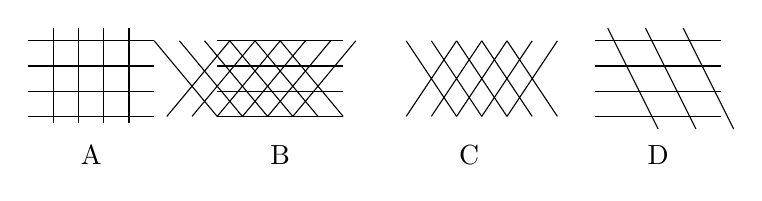
\begin{tikzpicture}[scale=.8]\foreach \y in {0,.4,.8,1.2}\draw(0,\y)--(2,\y);\foreach \x in {.4,.8,1.2,1.6}\draw(\x,-.1)--(\x,1.4);\node[below]at(1,-.3){A};\begin{scope}[xshift=3cm]\foreach \y in {0,.4,.8,1.2}\draw(0,\y)--(2,\y);\foreach \x in {-.8,-.4,0,.4,.8,1.2}\draw(\x,0)--++(1,1.2);\foreach \x in {0,.4,.8,1.2,1.6,2}\draw(\x,0)--++(-1,1.2);\node[below]at(1,-.3){B};\end{scope}\begin{scope}[xshift=6cm]\foreach \x in {0,.4,.8,1.2,1.6}\draw(\x,0)--++(.8,1.2) (\x,1.2)--++(.8,-1.2);\node[below]at(1,-.3){C};\end{scope}\begin{scope}[xshift=9cm]\foreach \y in {0,.4,.8,1.2}\draw(0,\y)--(2,\y);\foreach \x in {.2,.8,1.4}\draw(\x,1.4)--++(.8,-1.6);\node[below]at(1,-.3){D};\end{scope}\end{tikzpicture}
